\documentclass[11pt]{article}
\setlength{\oddsidemargin}{0in}
\setlength{\evensidemargin}{0in}
\setlength{\textwidth}{6.5in}

\usepackage{fancyhdr}
\usepackage{float}
\pagestyle{fancy}
\usepackage{amsmath,amsfonts,amssymb}
\usepackage{epsfig}
\usepackage{subfigure}
\usepackage{placeins}
\usepackage{amsmath}
\usepackage[usenames,dvipsnames,svgnames,table]{xcolor}
\usepackage{amssymb}
\usepackage{setspace}
\usepackage{graphicx} % Include figure files
\usepackage{times}
\usepackage{amsthm}
\usepackage{hyperref}
\usepackage{enumitem}
\hypersetup{bookmarks=true, unicode=false, pdftoolbar=true, pdfmenubar=true, pdffitwindow=false, pdfstartview={FitH}, pdfcreator={Daniel Larremore}, pdfproducer={Daniel Larremore}, pdfkeywords={} {} {}, pdfnewwindow=true, colorlinks=true, linkcolor=blue, citecolor=Green, filecolor=magenta, urlcolor=cyan,}
\usepackage[parfill]{parskip}

\usepackage{tcolorbox}
\tcbuselibrary{breakable}

\graphicspath{{../Notes/PythonFigs/}{./}}

\newcommand{\e}{\mathrm{e}}
\renewcommand{\d}{\mathrm{d}}
\newcommand{\erf}{\mathop\mathrm{erf}}
\newcommand{\erfc}{\mathop\mathrm{erfc}}
\newcommand{\xmin}{\ensuremath{x_{\min}}}
\newcommand{\ntail}{\ensuremath{n_{\rm tail}}}

\newcommand{\Q}[1]{\footnote{\textcolor{blue}{#1}}}

\begin{document}

\lhead{{\bf Mathematical \& Computational Modeling of Infectious Diseases \\ 
Homework 4}}
\rhead{{\bf D.B.\ Larremore\\2023}}
\renewcommand{\headrulewidth}{0.4pt}

{\bf Instructions:} 
\begin{itemize}[itemsep=-7pt]
	\item Please turn in a single PDF file. 
	\item Please share a link to your code, but do not attach the actual code. 
	\item Handwritten math (scanned and included in a PDF) is fine, but please watch out for 10MB+ file sizes!
\end{itemize}
\vspace{0.1in}\hrule

\begin{enumerate}
	\item The goal of this problem is to try out some of the methods we developed in class to estimate $R_0$ or $R_t$ from data. 
	
	{\bf What we know about Bison/Ralphie Unexplained Hiccups disease:}
	\begin{itemize}[itemsep=-5pt]
	\item BRUH disease affects bison like Ralphie.
	\item It is non-fatal, and does not affect mortality.
	\item Diagnosed via sporadic symptoms — mostly hiccups and bad breath.
	\item There are 100,000 bison in the herd
	\item Typical Bison lifespan in this herd is 100 weeks.
	\item Typical infection lasts 2 weeks, and a separate study found duration of infection exponentially distributed.
	\end{itemize}

	{\bf Weekly Incidence Data}
	\begin{itemize}[itemsep=-5pt]
		\item Weekly new case counts were recorded for ~10 years, which you can find on Canvas as {\bf all\_weeks.csv}.
		\item Ecologists believe they are identifying only 10\% of cases due to lack of funds.
		\item This 10\% ascertainment is an approximation — varies from week to week.
	\end{itemize}

	{\bf Prevalence and Seroprevalence Studies}
	\begin{itemize}[itemsep=-5pt]
		\item Ted Turner paid for a prevalence study to be done. A team of researchers went out into the field at night dressed in bison disguises, and subjected 1000 bison to tickling — a decent way to see if they have hiccups. Only 7 had hiccups. 
		\item The estate of Buffalo Bill paid for a seroprevalence study to be done. They took blood samples from 1000 randomly chosen bison and found that 517 had  BRUH antibodies.
	\end{itemize}
	
\begin{enumerate}[label=\alph*.]
	\item Estimate $R_0$ by examining the period of exponential growth (Method 1, Week 9). Be sure to show your work and plots as relevant. In the process, look up the 95\% confidence interval associated with estimating a slope from data points, and use the slope's confidence interval to provide a confidence interval for your $R_0$ estimate.
	
	\begin{tcolorbox}[breakable]
	\textbf{Solution}:\\
	We begin by using a method for estimating $R_0$ from the assumption that we are in the exponential growth regime of an outbreak. Starting from the canonical SIR with mortality (and incidentally, birthrate sufficient to keep a constant population), we have
	\begin{equation*}
		\dot{I} = \beta \frac{SI}{N}-(\gamma+\mu)I \approx (\beta-(\gamma+\mu))I,
	\end{equation*}
	where we have used the approximation that $I\approx N$ so most of the herd is susceptible. From here the approximate solution
	\begin{equation*}
		I(t)\approx I(0)e^{(R_0-1)(\gamma+\mu)t}=I(0)e^{(\beta-\gamma-\mu)t}
	\end{equation*}
	gives a method to approximate $R_0$ via 
	\begin{equation*}
		R_0\approx1+\frac{\hat{m}}{\gamma+\mu},
	\end{equation*}
	with $\hat{m}$ defined as the approximation of the slope extracted from data in log space. We take our estimations of $\gamma, \mu$ from literature (in this case presented in the problem statement) as 
	\begin{align*}
		\hat{\gamma} &= \frac{1}{2 \text{weeks}} = \frac{1}{2}[\text{weeks}^{-1}]\\
		\hat{\mu} &= \frac{1}{100 \text{weeks}}=\frac{1}{100}[\text{weeks}^{-1}].
	\end{align*}
	These values have some built in uncertainty from estimation and natural variation with time.\\
	\\
	A few things to note before we begin crunching numbers:
	\begin{enumerate}
		\item We need to be in an exponential growth region for this analysis to be valid. The provided data features large oscillations in the data which may indicate multiple waves, so for a reasonable estimate, I will subsample data from just the first wave.
		\item Exponential growth is, by nature, quite fast. For this reason, the number of data points available in the exponential growth region is quite small, which makes acurate data fitting tricky.
		\item For purposes of more advanced fitting techniques, the variance at each week is likely heteroskedastic, and dependent on the total infection load, making parameter estimation trickier.
	\end{enumerate}
	With this in mind, we begin by subsampling the data for the first 14 weeks of measurement. This is chosen due to the fact that the first 'wave' of infections appears to peak at around 20 weeks. We find using standard linear regression that the mean slope is $0.4872\ldots$ with a ci of $ [0.4561\ldots, 0.5184\ldots]$, leading to a mean estimate of $\hat{R_0}=1.925$ and CI of $[1.2326,2.0164]$
	
	\end{tcolorbox}

\begin{figure}
	\centering 
	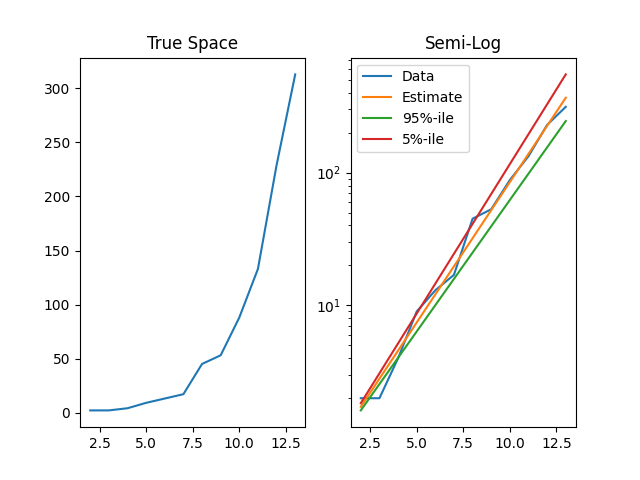
\includegraphics[scale = 1]{P1a.png}
	\caption{Data and comparison of linear regression in logspace.}
\end{figure}
	
	\item Estimate $R_0$ by utilizing the prevalence {\it or} seroprevalence data. (Method 2 or 4, Week 9). Be sure to show your work and plots as relevant. Write down (or look up) the 95\% confidence interval for the prevalence/seroprevalence estimate, and use it to provide a confidence interval for $R_0$.
	
	\begin{tcolorbox}[breakable]
	\textbf{Solution}:\\
	Before running the calculation of $\hat{R_0}$ from prevalence data, it is worth noting the that variance on $\hat{R_0}$ from prevalence data can be synthesized by, assuming independent sources of variance, as
	\begin{equation*}
		\hat{\sigma_{R_0}}^2 = \hat{R_0}^2\left((1+\frac{\gamma}{\mu})^2\sigma_{i}^2 + (\frac{i}{\mu})^2\sigma_{\gamma}^2+(\frac{i\gamma}{\mu})\sigma_{\mu}^2\right)
	\end{equation*}
	where $i, \gamma, \mu$ are interpreted as their estimated values. In this parameter regime, the variance in $\hat{R_0}$ is most sensitive to the variance in the equillibrium infections, which is small, and likely to have high variance. With that in mind, since Ted Turner's team reported 7 out of 1000 bison to have symptoms of the disease, the baysian MLE estimate gives
	\begin{equation*}
		\hat{\theta}=\frac{7}{1000+2}\approx 0.698\ldots\%
	\end{equation*}
	for prevalence in the population and is a surrogate for $i$ in the equation above. Then, converting $\theta$ into $R_0$ gives
	\begin{equation*}
		\hat{R_0}=\frac{1}{1-\hat{\theta}\left(\frac{\hat{\gamma}}{\hat{\mu}}+1\right)}\approx 1.553\ldots.
	\end{equation*}
	And to complete the calculation, the variance in $R_0$ should be roughly
	\begin{equation*}
		\widehat{\sigma_{R_0}}^2 \approx 18.155 \implies \widehat{\sigma_{R_0}} \approx 4.26
	\end{equation*}
	which throws the reliability of this estimate into question, but corroborates somewhat with the previous estimation of $\approx 1.925$
	\end{tcolorbox}
	
	\item (Grad / EC) Estimate $R_0$ a third way from the same data. 
	
	\begin{tcolorbox}[breakable]
	\textbf{Solution}:\\
		Here, we estimate from prevalence data. So we take a sample of the case near equillibrium. The last hundred weeks appear near equillibrium. Taking the $10\%$ estimate, the mean of $49.31$ cases becomes $493.1$, and the equillibrium density becomes $493.1/100000=0.004931$. Then, from given parameters, we get
		\begin{equation*}
			\hat{R_0}=\frac{1}{1-\hat{i}(\gamma/\mu-1)}=\frac{1}{1-0.004931(0.5/0.01-1)}=1.318.
		\end{equation*}
		This results is a much different and probably rather inaccurate since $\gamma/\mu=50$ is rather large. 
	\end{tcolorbox}
	
	\item Compare your estimates, the uncertainty associated with each, and discuss what might cause them to be different.
	
	\begin{tcolorbox}[breakable]
	\textbf{Solution}:\\
		Between the seroprevalence method and exponential fitting method, the seroprvalence method gives a much larger confidence interval than the exponential fitting method, but their mean estimates are actually quite close, relatively speaking. It is worth noting that the $R_0$ value is not necessarily static in time, and the data used are all from different time periods. 
	\end{tcolorbox}
	
	\item (EC for all) Estimate $R_t$ using Method 5.
	
	\begin{tcolorbox}[breakable]
	\textbf{Solution}:\\
		
	\end{tcolorbox}
	
\end{enumerate}

\clearpage
\item The goal of this problem is to get some simple practice with sensitivity and specificity. 

Suppose we've got a diagnostic with sensitivity $0.90$ and specificity $0.98$. 

\begin{enumerate}[label=\alph*.]
	\item Maria Lara conducts a prevalence study with the above diagnostic. She samples 100 people and gets 39 positives. What is your estimate of the prevalence after correcting for the sensitivity and specificity? 
	
	\begin{tcolorbox}[breakable]
		\textbf{Solution}:\\
		We take the naieve estimate of the rate of positives as 
		\begin{equation*}
			\hat{\phi}=\frac{39}{100}=0.39
		\end{equation*}
		and solve for prevalence from 
		\begin{equation*}
			\hat{\theta}=\frac{\hat{\phi}-(1-sp)}{se+sp-1}=\frac{0.39-0.02}{0.88}=0.42
		\end{equation*}
	\end{tcolorbox}
	
	\item Write down a 95\% confidence interval for your corrected estimate. 
	
	\begin{tcolorbox}[breakable]
		\textbf{Solution}:\\
		The estimate of the postitive rate is taken as the mean of the number of positives in the sample. So the CI on $\hat{\phi}$ is simply
		\begin{align*}
			[\hat{\phi}-0.96\sqrt{\frac{\hat{\phi}(1-\hat{\phi})}{N}}, \hat{\phi}-0.96\sqrt{\frac{\hat{\phi}(1-\hat{\phi})}{N}}] &\approx [0.39-0.0955, 0.39+0.0.0955]\\
			&\approx[0.2944, 0.4855].
		\end{align*}
		Carrying thes bounds through to $\hat{\theta}$ since the specificity and sensitivity are not interpreted as random variables, we have
		\begin{equation*}
			CI(\hat{\theta})\approx [0.42\pm 0.1086] \approx [0.3113,0.5286]
		\end{equation*}
	\end{tcolorbox}
	
	\item Trying to be helpful, Burt Q. Losis conducts a second prevalence study in the same population and finds 18 positives out of 50 samples. Again estimate the prevalence and a 95\% confidence interval.
	
	\begin{tcolorbox}[breakable]
		\textbf{Solution}:\\
		We repeat the above. The estimate of the rate of positives in the population is 
		\begin{align*}
			\hat{\phi} &= 0.36\\
			CI(\hat{\phi})&=[0.36\pm 0.1330]\approx[0.2230, 0.4930].
		\end{align*}
		Carrying it through the sensitivity/specificity corrected prevalence formula gives
		\begin{align*}
			\hat{\theta}\approx 0.3863\\
			CI(\hat{\theta})\approx [0.3863\pm 0.1511]\approx [0.2352, 0.5374]
		\end{align*}
		as needed.
		
	\end{tcolorbox}
	
	\item Pool Burt's and Maria's data to get a third estimate of prevalence, and update your 95\% confidence interval. How are your three estimates related? And, how are the widths of the three confidence intervals related? 
	
	\begin{tcolorbox}[breakable]
		\textbf{Solution}:\\
		We take the assumption that Burts and Marias data are from identical distributions and uncorreleted. Then, we may simply pool data together for an effective population of $N=150$ and we see $57$ positives. Then, repeating calculations yields
		\begin{align*}
			\hat{\phi} &=0.38\\
			CI(\hat{\phi}) &\approx [0.38\pm 0.0777] \approx [0.3023, 0.4577].
		\end{align*}
		
		Carrying through to prevalence gives
		\begin{align*}
			\hat{\theta}&\approx 0.4091\\
			CI(\hat{\theta})&\approx [0.4091\pm 0.0883] \approx [0.3208,0.4974],
		\end{align*}
		as needed. We have the range of the three estimates are $0.2172, 0.3022, 0.1766$ for Maria, Burt, and the pooled data respectively. We note that Burts range is largest since he had the smallest sample size, Maria's next, and the pooled data has the smallest confidence interval of the three.
	\end{tcolorbox}
	
	\item (Grad / EC) You test yourself. Positive! What is your best guess of the probability that you are {\it actually} positive?
	
	\begin{tcolorbox}[breakable]
		\textbf{Solution}:\\
		Taking the parameters from before, we note that 
		\begin{align*}
			PR(actually +|test +) &\approx \hat{\theta}se + (1-\hat{\theta})(1-se) \\
			&\approx (0.4091)(0.9)-(0.5909)(0.02) \approx 0.380008\ldots
		\end{align*}
		which puts the probability that I am actually positive very close the estimate for positivity rate, as one may expect.
	\end{tcolorbox}
	
\end{enumerate}

\clearpage

\item The goal of this problem is to learn about how sensitivity and specificity arise from calibration data, i.e. from positive and negative controls. For this problem, you will need to read in three .csv files to access the data they contain:
\begin{itemize}
	\item {\bf HW4\_Q3\_neg.csv}: The assay values associated with a set of negative controls. 
	\item {\bf HW4\_Q3\_pos.csv}: The assay values associated with a set of positive controls. 
	\item {\bf HW4\_Q3\_data.csv}: The assay values associated with your prevalence study in the population.
\end{itemize}
\vspace{0.5in}

\begin{enumerate}[label=\alph*.]
	\item Read in the data and produce a tall, skinny plot with three columns of data: the negative controls (red), the positive controls (black), and the data from the field (blue). Use jitter and transparency (``alpha'') to allow us to see the distributions of the data. 
	
	\begin{tcolorbox}[breakable]
		\textbf{Solution}:\\
		Here is my plot in Fig. \ref{fig:posneg}
	\end{tcolorbox}
\begin{figure}
	\centering
	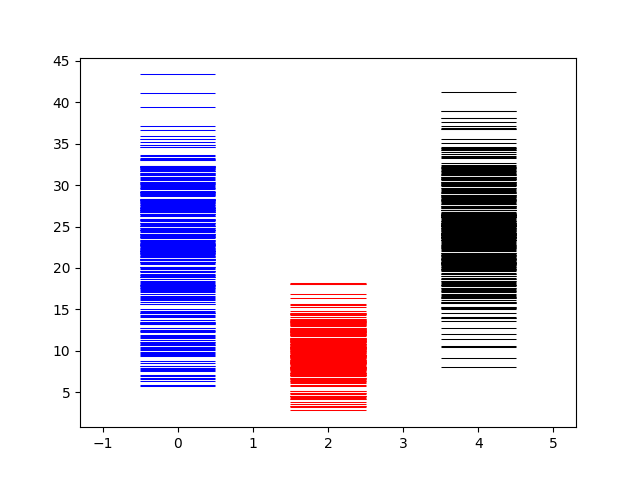
\includegraphics{p3p1.png}
	\caption{Data in blue, negative controls in red, positive controls in black.}
	\label{fig:posneg}
\end{figure}
	
	\item Consider a cutoff $c$ such that any assay values above $c$ are to be called positive and any assay values below $c$ are to be called negative. Then write four functions: $se(c)$, $sp(c)$, and $\hat{\phi}(c)$ and $\hat{\theta}(c)$. They should correspond to the sensitivity, the specificity, the raw prevalence in the field data, and the corrected prevalence in the field data. What value of $c$ corresponds to the ``Youden'' choice?
	
	\begin{tcolorbox}[breakable]
		\textbf{Solution}:\\
		Code provided in my github link. The Youden choice maximizes the sum of specificty and sensitivity minus 1, this appears to hit a maximum at $c=15, Y(c)=0.92$
	\end{tcolorbox}
	
	\item (Grad / EC) By sweeping over various choices of $c$, plot a receiver operator curve, and place a point at the Youden choice. Create a second plot showing how $\hat{\theta}(c)$ varies, and again, place a point at the Youden choice. 
	
	\begin{tcolorbox}[breakable]
		\textbf{Solution}:\\
		Plots can be seen in Figs \ref{fig:roc}, \ref{fig:corr_prev} for ROC and corrected prevalence values respectively.
	\end{tcolorbox}

	\begin{figure}
		\centering
		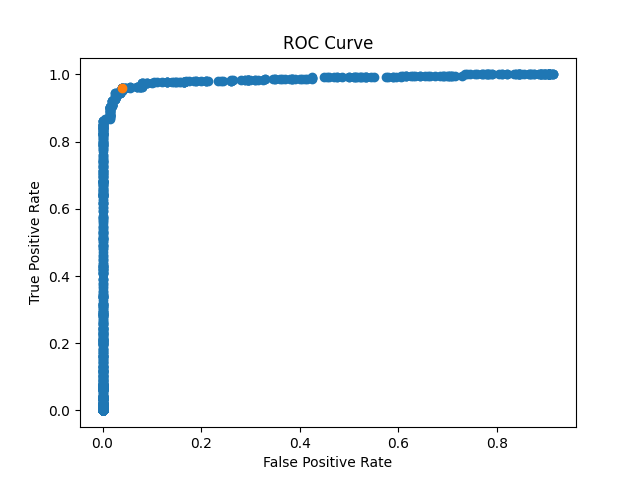
\includegraphics{roc.png}
		\label{fig:roc}
		\caption{Youden point is the orange dot.}
	\end{figure}

	\begin{figure}
	\centering
	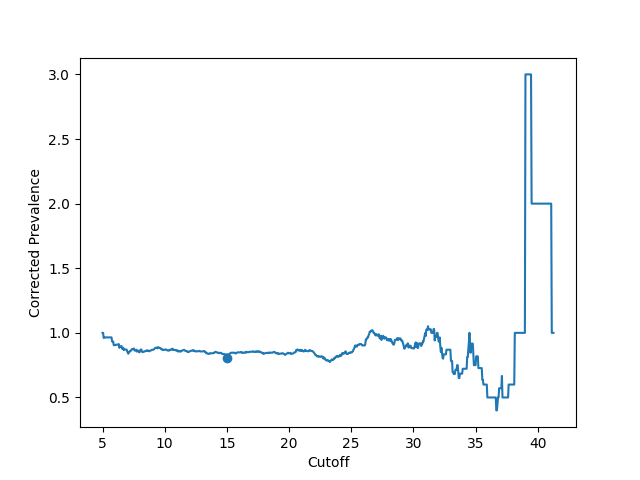
\includegraphics{PrevOverCutoff.png}
	\label{fig:corr_prev}
	\caption{Youden point is the blue dot. For larger cutoffs, corrected prevalence deviates wildly outside of $(0,1)$}
\end{figure}
	
	\item Write 3-4 sentences reflecting on how the conclusions of a study might be affected by how one decides to choose the cutoff at which positives and negatives are called. 
	
	\begin{tcolorbox}[breakable]
		\textbf{Solution}:\\
		When desiging a test for a study to estimate important epidemiologic factors, like disease prevalence, the cutoff parameter can greatly effect the results. For example, prevalence in the data can vary between as much as 1 and as little as 0.5 when it is valid. These give very different pictures of the progress of an epidemic in terms of its progress and severity. Careful and well motivated decisions about test design are crucial to getting an acurate and meaningful picture of an epidemic.
	\end{tcolorbox}
	
\end{enumerate}

\end{enumerate}


\end{document}